%%%%%%%%%%%%%%%%%%%%%%%%%%%%%%%%%%%%%%STARt PREAMBLE
\documentclass{article}

%Required: You must have these
\usepackage{Sweave}
\usepackage{graphicx}
\usepackage{tabularx}
\usepackage{hyperref}
\usepackage{natbib}
\usepackage{pdflscape}
\usepackage{array}
\usepackage{authblk}
\usepackage{gensymb}

%\usepackage[backend=bibtex]{biblatex}
%Strongly recommended
 %put your figures in one place
%\SweaveOpts{prefix.string=figures/, eps=FALSE} 
%you'll want these for pretty captioning
\usepackage[small]{caption}

\setkeys{Gin}{width=0.8\textwidth} %make the figs 50 perc textwidth
\setlength{\captionmargin}{30pt}
\setlength{\abovecaptionskip}{10pt}
\setlength{\belowcaptionskip}{10pt}
% manual for caption http://www.dd.chalmers.se/latex/Docs/PDF/caption.pdf

%Optional: I like to muck with my margins and spacing in ways that LaTeX frowns on
%Here's how to do that
\topmargin -1.5cm  
\oddsidemargin -0.04cm 
\evensidemargin -0.04cm % same as oddsidemargin but for left-hand pages
\textwidth 16.59cm
\textheight 21.94cm 
%\pagestyle{empty}  % Uncomment if don't want page numbers
\parskip 7.2pt   % sets spacing between paragraphs
%\renewcommand{\baselinestretch}{1.5} 	% Uncomment for 1.5 spacing between lines
\parindent 0pt% sets leading space for paragraphs
\usepackage{setspace}
%\doublespacing
\renewcommand{\baselinestretch}{1}
\usepackage{lineno}
 
%%%%%%%%%%%%%%%%%%%%%%%%%%%%%%%%%%%%%%END PREAMBLE 

%Start of the document
\begin{document}

%\SweaveOpts{concordance=FALSE}
\Sconcordance{concordance:bayes4cons_doc.tex:bayes4cons_doc.Rnw:1 310 1}


\bibliographystyle{bibstyles/amnat.bst}
\title{Benefits of Bayesian Modelling For Conservation} 
\author[1,a]{A.K. Ettinger}
\author[2]{H. Eyster}
\author[3]{D. Loughnan}
\author[3]{X. Wang}
\author[3]{E.M. Wolkovich}
\author[3]{M. Auger-Methe}
\author[4]{R. Zenil-Ferguson}
\author[5]{V. Leos Barajas}
\author[6]{Leithen M'Gonigle}
\author[6]{Hanna Jackson}
\author[7]{Others from Symposium working group?}


\affil[1]{The Nature Conservancy,Seattle, Washington, USA}
\affil[2]{TNC}
\affil[3]{UBC}
\affil[4]{UKY}
\affil[5]{University of Toronto}
\affil[6]{SFU}
\affil[7]{Multiple other institutions?}


\affil[a]{Corresponding author; email: ailene.ettinger@tnc.org; mailing address: 74 Wall Street. Seattle, WA 98121, USA }

\date{\today}
\maketitle 
\textbf{Author contributions}: All authors conceived of this manuscript, which began at a Bayesian Generative Modelling Symposium at University of British Columbia in 2024, and all authors contributed to manuscript revisions.

\textbf{Data Accessibility} 

\textbf{Running title} 

\textbf{Key words} 


\textbf{Paper type} Review or Perspective in Frontiers in Ecology and the Environment, Conservation Biology, Conservation Letters, or Conservation Science and Practice

\textbf{Focal Audience} Conservation biologists and other scientists who would like to influence conservation/environmental policy, IPCC 



%%%%%%%%%%%%%%%%%%%%%%%%%%%%%%%%%%%%%%%%%%%%%%%%%%%

%%%%%%%%%%%%%%%%%%%%%%%%%%%%%%%%%%%%%%%%%%%%%%%%%%%

%\linenumbers

\section*{Abstract} 


\newpage
\section* {Introduction: The challenges and needs of today's conservation science are well-suited for Bayesian data analysis}

\par Conservation science in the 21st century seeks to address the dual crises of  climate change and rapid biodiversity loss. These are problems that require urgent action globally, as loss of earth's biodiversity and its benefits are accelerating \citep{brondizio2019assessing, ripple2017extinction,tittensor2014mid}. Conserving biodiversity is, of course, the primary motivation for the field of conservation biology \citep{williams2020past} and at the heart of recent international resolutions such as the Convention on Biological Diversity's Aichi targets (UNEP CBD 2010) and of Sustainable Development Goal 15 \citep{assembly2015resolution}. 
\par Recently, nature conservation has been integrated into global climate change mitigation assessment and efforts, as well, through the concept of ‘natural climate solutions’ (NCS). NCS are intentional human actions (or 'NCS pathways') that protect, restore, and improve management of forests, wetlands, grasslands, oceans, and agricultural lands to mitigate climate change \citep{griscom2017natural}.

\par Though action is urgently needed, effective biodiversity conservation and durable climate change solutions should be evidence-based. 
\begin{itemize}
\item 'best available science' often required by  policy
\item part of science process, though often 'ideal' data are not available
\item synthesizing multiple data sources  and incomplete datasets may be required 
\end{itemize}

\par 
\par A critical part of building the evidence base is transparency and reproducibility in science. 
\begin{itemize}
\item This includes being transparent and clear about uncertainty
\item Communicating/quantifying uncertainty about climate change mitigation (e.g., principles of Natural Climate Solutions, Ellis 2023, IPCC requires uncertainty (Chap 3 from 2006))

\end{itemize}
\par 
\par Bayesian data analysis provides a framework and approaches that align well with these needs of conservation biology.

\begin{itemize}

\item Moving beyond null-hypothesis testing 
\item Propagation of uncertainty
\item Frameworks to synthesize multiple sources of data and update as new information becomes available
\item Though some fields within conservation biology and natural resource management have adopted Bayesian methods (wildlife mark and recapture models or occupancy models, fisheries), historically they have not been widely used conservation science.

\end{itemize}

\subsection*{Aim} We aim to help accelerate adoption of Bayesian data analytical approaches in conservation science because we believe these approaches offer features that are well-suited to the field and could enhance progress, with more  widespread adoption. We describe the benefits of using Bayesian methods for conservation science questions, summarize what is required to use these methods, and provide example code and analyses relevant to current conservation problems. We also share resources and a glossary that we hope will make Bayesian tools more approachable to those who have not used them before.

\section* {Benefits for Conservation}
\subsection*{Bayesian approaches offer powerful and flexible model that can get the job done!}
\par Ecological data are notoriously poorly aligned with classic stastical techniques (e.g., nonnormal data, unbalanced, etc). This can result in situations where frequentist models are not possible to fit or result in inaccurate estimates (e.g.,case study 1). Bayesian modelling approaches are flexible and powerful enough to provide robust estimates under a wide range of conditions. 
\par In addition, conservationists are often particularly interested in species with small populations, since these are often the ones most at risk of extinction, or ones that are poorly understood \citep{stinchcombe2002influence}. Frequentist statistics rely on asymptotic behavior, which makes it difficult for these methods to draw useful conclusions from small sample sizes \citep{mcneigh2016using}. Bayesian methods, however, do not have this same reliance, and so are better able to accommodate small sample sizes. However, these methods still require care when working with small sample sizes, because priors matter much more; yet this is also an opportunity to include the full gamut of prior knowledge from many sources that may not typically be included in quantitative analyses \citep{mcneish2016using}. 

\subsection*{Frameworks for integrating multiple data sources}
\par Conservation problems are complex and addressing them, especially in the era of climate change, requires integrating social, economic, biological, and physical information to provide the evidence base upon which decisions can be made. Conservation evidence comes in many forms, including from quantitative studies, community knowledge, expert knowledge, traditional ecological knowledge, and others. Conservation decision-making requires integrating these multiple sources of information to provide an evidence base upon which decisions can be grounded \citep{stern2022interweaving}. Bayesian methods enable two fruitful avenues for such integration. First, information can be amalgamated into Bayesian Belief Networks \citep{marcot2001using,newton2007bayesian}. Second, extant information can be used to inform prior distributions \citep{o2008informed}. 

\subsection*{Adaptive management and comparing alternatives}
\par Conservation scientists often need to compare outcomes from current 'business-as-usual' approaches to new alternatives. For example, conservation scientists might be interested in deciding whether an alternative practice produces the same results as current practice. 
The need to test new approaches, coupled with the fact that ecosystems are dynamic and often yield unexpected behaviors \citep{Levin2012,Gross2013}, have led to practices of adaptive management in conservation \citep{holling1978adaptive}. Yet frequentist statistical frameworks rarely provide information necessary to inform adaptive management  \citep{prato2005bayesian}.  Specifically, frequentist statistics incapacity to compare support for a variety of hypotheses (including a 'null' hypothesis) prevents this method from informing what interventions will most likely bring about conservation gains \citep{prato2005bayesian}. For example, in its submission process, leading conservation journal \textit{Conservation Biology} requires that authors recognize that, ``8. ensured you have not misinterpreted statistical nonsignificance as no effect if a frequentist approach was used (absence of evidence is not evidence of absence)?'' Bayesian analysis, on the other hand, can provide evidence to support a null hypothesis, e.g., that the current and alternative and current management practices produce similar results \citep{gallistel2009importance}.
\subsection*{Ability to quantify and propagate uncertainty} 
\par Bayesian analyses are particularly useful for decision-making because they not only include a range of information types, but also include associated uncertainty \citep{stern2022interweaving}. The integration of multiple datasets required by many conservation problems in turn necessitates quantifying and sometimes propoagating uncertainty across multiple sources and/or multiple modeling steps. Bayesian approaches enable straightforward quantification and  propagation of  uncertainty, including for some conservation problems that can require analyses for which frequentist statistics are unable to compute the associated uncertainties \citep{bolker2009a,bates2006r}. Frequentist statistics produce metrics like confidence intervals and p-values, which have very specific interpretations \citep{fornacon2021bayesian}. However, these metrics are often misinterpreted. Bayesian statistics, in contrast, produces credible intervals, for which the intuitive interpretation matches the technical definition, yielding much more easily interpretable results, particularly for non-statistician colleagues and decision-makers (Fornacon-Wood, 2021). 
\par Moreover, Bayesian methods enable uncertainty to be propagated through multiple analyses, ensuring that end results represent the full uncertainty of the process under study. \citep{draper1995assessment,gilbert2023propagating,Eyster2022,Saunders2019}. For example, using Bayesian methods, one can calculate the abundance of birds in different types of management landscapes such as traditional agriculture and perennial polycultures, and then propagate the uncertainty associated with those abundances into a downstream analysis to test whether the bird communities in the alternative perennial polyculture landscape are maintained simply as an ecological sink \citep{Eyster2022}. 


\par Conservation often requires making easily-interpretable wildlife status categories to inform decision making (Brooks, 2008). For example, conservation might be prioritized for species declining 'rapidly' versus 'moderately.' These discrete categories require information about when a species' population has passed a particular threshold (Brooks, 2008).  Bayesian models make it possible to assess the evidence for whether a species has surpassed a given threshold (Brooks, 2008). 


\section* {Case Studies}
\subsection*{Robust estimates; bird example (Deirdre, Mao)}
\begin{itemize}

\item Extinction example referenced in \citep{wade2000bayesian}. Compare frequentist (Maximum likelihood) to Bayesian analysis to get at population trend and extinction risk 
\item simulate data
\end{itemize}

\subsection*{Propagating uncertainty; NCS example (Ailene)}
\begin{itemize}
\item Mitigation= flux X extent
\item uncertainty propogation using posterior
\item compare to boot-strapping 
\end{itemize}

\section* {A future with more widespread use of Bayesian modelling in Conservation}
\begin{itemize}
\item Implementing Bayesian modelling is easier than ever before! Computational resources (add some details)- are getting easier and should continue getting easier to develop, test, and refine models that represent focal systems and are able to address relevant questions)
\item Urgency and complexity of problems and systems requires flexible, powerful modelling appraoches 
\item We envision a future in which conservation and ecology students (undegraduate and graduate levels) recieve statistical training to provide strong foundations in Bayesian statistics. Currently the focus of many introductory statistics classes is frequentist methods, which are not appropriate for most ecological data. It doesn't have to be this way! 
\item IPCC and other global institutions should include guidelines for Bayesian approaches increasibly used by ecologists ( Fig. 1), as NCS gets integrated into the climate/biophysical analyses that dominated early IPCC work.
\end{itemize}

\par 
\section* {Box 1: Defining Bayesian Analysis}

\section* {Box 2: Resources to Get Started}

\bibliography{conslib.bib}

\section* {Figures}

\begin{figure}[h]
\centering
 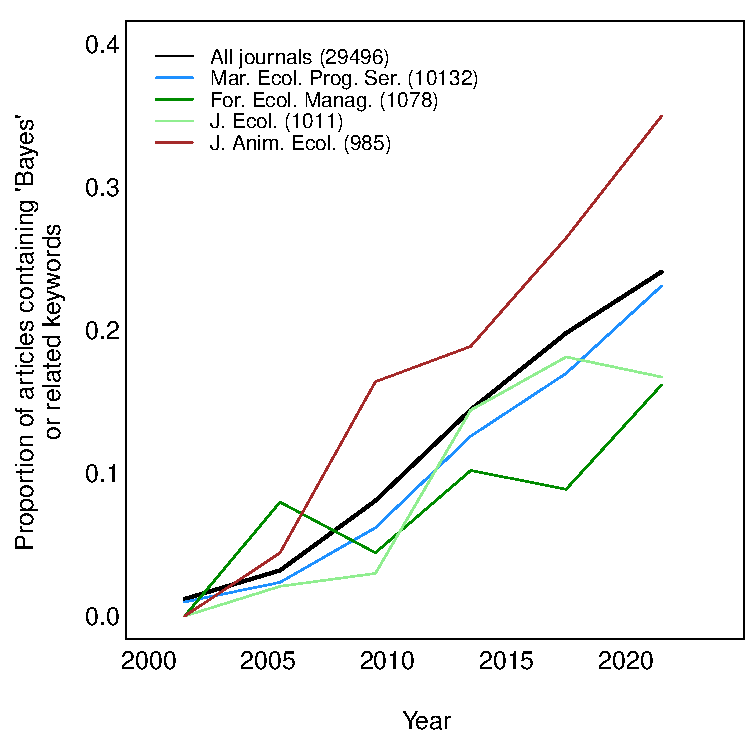
\includegraphics{../figs/conservation.pdf}
 \caption{\textbf{Proportion papers using Bayes in XX major conservation journals since 2000}} 
 \label{fig:consbaystrend}
 \end{figure}
 
 \begin{figure}[h]
\centering
 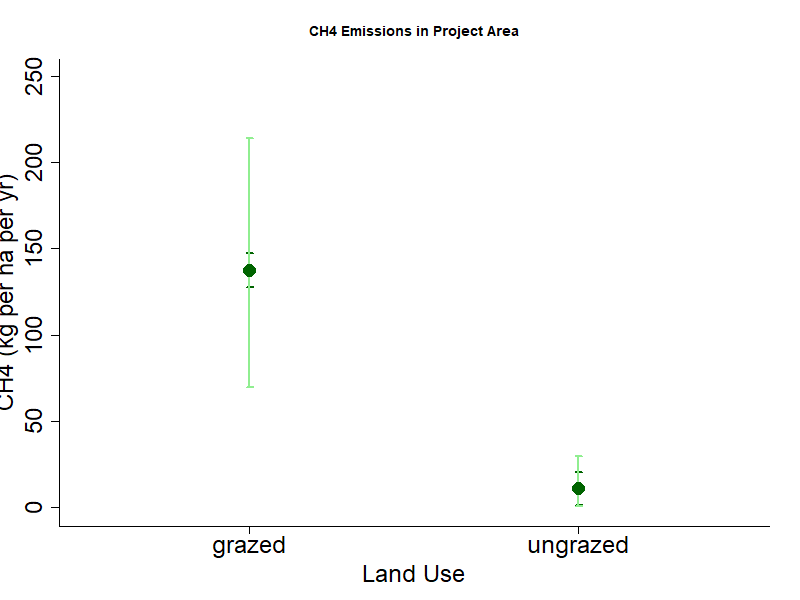
\includegraphics{../figs/ncs/ncsprojimpactch4.png}
 \caption{\textbf{NCS Example: Uncertainty propagation}} 
 \label{fig:ncs}
 \end{figure}
%%%%%%%%%%%%%%%%%%
%%%%%%%%%%%%%%%%%%%%%%
\end{document}
%%%%%%%%%%%%%%%%%%%%%%%%%%%%%%%%%%%%%%%%

